% !TeX program = xelatex
\documentclass{vilgym}

% For math
\usepackage{mathtools}
\usepackage{amsfonts}

% For graphs
\usepackage{graphicx}

% General info
\title{Kunsti genereerimine teksti põhjal}
\author{Karl-Joan Alesma, III MF}
\instructor{õp Malle Eglit}
\date{2019}

% Define expected value operator
\DeclareMathOperator{\EX}{\mathbb{E}}
\DeclareMathOperator{\loss}{\mathcal{L}}
\DeclarePairedDelimiter{\norm}{\lVert}{\rVert}

\DeclareNameAlias{sortname}{family-given}
\addbibresource{viited.bib}
%\DeclareNameAlias{sortname}{family-given}

\usepackage{xpatch}

% Remove parenthesis around year
\xpatchbibmacro{date+extradate}{%
  \printtext[parens]%
}{%
  \setunit*{\space}%
  \printtext%
}{}{}


\begin{document}
	\maketitle
	\tableofcontents

	%\unsection{Definitsioonid}
	%\begin{description}
	%\let\originalitem\item
	%\renewcommand*{\item}[1][]{\originalitem[#1]\label{def:#1}}

	%\item{GAN} ing.k. \textit{generative adversarial network}
	%\end{description}

	%\newcommand*{\seedefinition}[1]{(\hyperref[def:#1]{vt~definitsiooni})}
	\newcommand*{\ingk}[1]{(\textit{ing. k. #1})}

	\unsection{Sissejuhatus}
	Sügavõppe \ingk{Deep Learning} on meetodite kogu, mis võimaldab õppetada arvutile, kuidas lahendada erinevaid probleeme. Antud disipliin on eksisteerinud juba alatest 1940 aastatest (küll aga teise nime all), kuid on alles hiljuti kasvanud populaarsuses. Kiiret arengut ja edasi minekut on peamiselt põhjustanud kaks asja: arvuti ressursside kasv ning järjest suurenev andmete hulk. Need kaks asja on võimaldanud treenida sügavamaid, keerulisemaid ning täpsemaid mudeleid. \parencite{deeplearningbook}	 

	Üks uus mudel, mis on kiire kasvuga tekkinud, on GAN ehk generatiivne adverstiivne võrk. Antud võrku on võimalik treenida jäljendama erinevaid andme distributsioone. Kasutades treenimise käigus õpitud representatsioone, suudab too võrk genereerida uut materjali, mis on sarnane treenimisel kasutatud andmetega. \parencite{gan}

	Uurimistöö eesmärk on luua mudel kasutades GANe, mis on ise võimeline genereerima kunsti teksti põhjal. Andes mudelile sisendiks kirjelduse, milline peab olema loodava kunstiteose sisu ja mis stiilis, genereerib mudel teose, mida tegelikkuses ei eksisteerigi. Lisaks saab autor selle protsessi käigus kinnitada ja laiendada oma teadmisi sügavõppest.

	Kuna puuduvad digitaalsed andmekogud, kus oleksid olemas teoste kirjeldused (nt "Pildil on mees, kes raiub puid, ning tema selja taga on karu"), ei ole võimalik treenida ühte GANi, mis suudaks teisendada sisu kirjelduse kunstiteoseks. Selleks kasutab autor kahte GANi --- esimene GAN teisendab sisu kirjelduse vastavaks pildiks (sisu\textrightarrow pilt), mis antakse järgmisele GANile, mis muudab loodud pildi kunstiteoseks soovitus stiilis (pilt\textrightarrow kunst).

	Hüpotees on, et mudel, mis on treenitud genereerima ainult ühte kindlat objekti sisaldavaid teoseid (ehk mudel suudab luua teoseid, kus on näiteks ainult linnud), loob realistlikumaid teoseid kui mudel, mis on treenitud genereerima mitmeid erinevaid objekte sisaldavaid teoseid (ehk mudel suudab luua teoseid, kus on näiteks majad, metsad või muu selline).

	Töö alguses annab autor ülevaate varasematest töödest selles valdkonnas ning tutvustab loogikat, mille põhjal on mudel kokkupandud. Seejärel tutvustatakse erinevaid mudeleid, millele järgneb eksperimentaalne osa, kus analüüsitakse ning hinnatakse erinevate mudelite sooritust. 
	
	\section{Varasemad tööd}

	Uue materjali genereerimine on keeruline probleem. Kogu sügavõppes ajaloo vältelt on diskrimineerivad mudelid saavutanud paremaid tulemusi kui generatiivsed mudelid. Hiljuti on aga see muutunud GANide tekkega \parencite{gan}. GANid on saavutanud märkimisväärseid tulemusi pildi \parencite{biggan} ja video generatsioonis \parencite{dvdgan} ning saanud hakkama ka pildi resolutsiooni suurendamise ehk super resolutsiooniga \parencite{srgan}. GANide edu põhjuseks on kahe närvivõrgu omavaheline võistlus, mille tulemusel genereeritud materjali kvaliteet paraneb ideaalis seni, kuni on eristamatu päris materjalist, mida GAN püüab järele aimata. GANi tööpõhimõttet tutvustatakse järgmises peatükkis.

	Pildi genereerimine tekstist on huvitav probleem, mille arengus on hoogu andnud GANide kasutusele võtt. Reed jt kasutasid sisendist sõltuvat GANi \ingk{conditional GAN}, millele anti sisendiks tekstist närvivõrguga eraldatud sisu, et genereerida 64x64 suurusega pilte \parencite{reed}. Nende järgmine töö kasutas peale tekstisisendi ka objekti asukohta, mis parandas loodud piltide kvaliteeti \parencite{reed2}. 

	Zhang jt kasutasid kahte GANi, et genereerida parema resolutsiooniga pilte. Esimene GAN genereerib ligikaudse visandi, millele teine GAN lisab detaile ning suurendab resolutsiooni \parencite{stackgan}. Antud lähenemine on lihtsam kui pildi genereerimine ühe GANiga. Nende järgmine töö kasutas kolme GANi, mis olid üksteise otsa pandud, et genereerida järjest suurema resulutsiooniga pilte. Esimene generaator genereeris pilte suurusega 64x64, teine 128x128 ja kolmas 256x256 \parencite{stackgan2}.

	Xu jt mudel AttnGAN kasutab samuti 3 GANist koosnevat struktuuri, aga millele on juurde lisatud tähelepanumehanism \parencite{attngan}. Tähelepanu võimaldab mudelil joonistada erinevaid alamregioone keskendudes sõnadele, mis on antud piirkonna jaoks kõige olulisemad. Kasutan oma mudelis Xu jt mudelit komponendina, mis muudab sisu kirjelduse pildiks (sisu\textrightarrow pilt), kuna antud mudeli tulemused on teiste omadest paremad. 

	Selleks, et muuta tavaline pilte kunstiteoseks, on kaks erinevat võimalust --- stiili ülekanne või CycleGAN. Stiili ülekanne võtab sisendiks sisupildi ja stiilipildi ning proovib seejärel genereerida pildi, mille sisu on sarnane sisupildiga ja mille stiil on sarnane stiilipildiga \parencite{styletransfer}.
	Selleks kasutatakse varem treenitud pildid klassifitseerija erinevaid kihte, et mõõta kahe pildi vahelist sisu ja stiili sarnasust. 

	CycleGAN võimaldab treenida see-eest GANi, mis teisendab sisendpildi ühest domeenist teise. Näiteks mustvalge pilt värviliseks, sebra hobuseks või antud juhul pildi kunstiteoseks. Treenimise käigus kasutadakse põhimõtted, et kui muuta mustvalge pilt värviliseks, siis saadud värvilise pildi teisendamisel mustvalgeks, peaks jõudma tagasi algse musta pildini. \parencite{cyclegan}

	Kui võrrelda CycleGANi ja stiili ülekannet, siis stiil ülekande puudujäägiks on tema võime ainult teisendada ühe pildi stiil teisele pildid, samas kui CycleGAN suudab teisendada terve piltide kollektsiooni stiili soovitud pildile. Zhu jt on ka leidnud, et Gatys jt meetodil ei õnnestu tihti luua fotorealistlikke pilte \parencite{cyclegan}. Kasutan oma mudelis CycleGANi komponendina, mis muudab pildi soovitud stiiliga teoseks (pilt\textrightarrow kunst), kuna antud mudel suudab kanda üle terve kollektsiooni stiili ning luua realistlikkemaid pilte.

	Leidub varasemaid töid, kus on kasutatud GANi, et genereerida kunsti, näiteks ArtGAN\parencite{artgan}, GANGough\parencite{gangough} ja CAN\parencite{can}. Need mudelid kasutavad valdavalt ühte tingivat GANi ($ F(\boldsymbol{z}|\boldsymbol{\theta}) $, $ \boldsymbol{z} $ on müravektor ja $ \boldsymbol{\theta} $ on stiilivektor), mis võimaldab genereerida erinevas stiilis ja sisuga teoseid. Sellise viisi puhul saab muuta loodavat sisu muutes vektorit $ \boldsymbol{\theta} $, mis muudab peamiselt loodava teose stiili ja seega loodavat sisu, aga ei võimalda täpselt määrata loodava teose sisu. 

	Antud töö autori viisiga on teoreetilselt võimalik kontrollida teose sisu ja stiili ning mille puhul on ka samast sisendist genereeritud teosed erinevad. Kuna puuduvad andmed kunstiteoste ja nende kirjelduste vahel, ei saa genereerida kunsti, mille sisu saab kirjeldusega määrata, ainult ühe GANiga. Seega koosneb autori mudel 2 GANist --- AttnGANist (sisu\textrightarrow pilt) ja CycleGANist (pilt\textrightarrow kunst). %, mida edaspidi nimetan text2art-ganiks.


	%  \section{Mudel}
	\section{Tehnilised detailid}
	Eelmises osas anti põgus ülevaade erinevadest mudelidest. Selles osas kirjeldatakse põhjalikumalt, kuidas töötab GAN, AttnGAN ja CycleGAN.

	\subsection{GAN}
	Generatiivne adversatiivne võrk ehk GAN \ingk{generative adversarial network} on sügavõppe mudel, mis koosneb kahest neruonvõrgust --- üks on diskrimineerija \ingk{discriminator} ja teine on generaator \ingk{generator}.  Generaatori ülesandeks on luua sisu, mis on sarnane kasutusel olevate andmete distributsiooniga. Diskrimineerija ülesandeks on määrata, kas talle näidatud sisu on võetud päris andmete hulgast või on loodud generaatori poolt.
	
	Generaatoril ja diskrimineerijal vastastikused ülesanded --- diskrimineerija proovib minimeerida viga, mis tehakse sisu klassifitseerimise käigus (kas on võetud päris andmete hulgast või loodud generaatori poolt), ja generaator proovib maksimeerida viga, mida diskrimineerija teeb klassifikatsiooni käigus. Kokkuvõtvalt need kaks võrku mängivad omavahel minimaksmängu \ingk{minimax}, mida võib võrrelda vägikaika veoga. Lõpuks jõutakse Nash tasakaalu \ingk{Nash equilibrium}, kus osalejatel ei ole enam midagi saada oma strateegia muutmisega \parencite{gametheory}. Ideaalis on sel juhul diskriminaatori poolt väljastatud tõenäosus sõltumata sisendist $ 1/2 $.

	Ilustavalt võib mõelda generaatorist kui võltsjate meeskonnast, kes proovivad luua võltsraha ja kasutada seda ilma jäljeta. Diskrimineerija aga käitub kui politsei, proovides tuvastada kas tegu on võltsinguga. Alguses on võltsjatel võltsingud kehvad ning politseil on raskusi tuvastusega, aga aja jooksul muutuvad osapooled paremaks omavahelise võistluse tõttu, kuni hetkeni mil võltsingud pole enam eristatavad päris valuutast.

	Treenimis protsetuuri saab võtta kokku järgimse funktsiooniga:

	\begin{equation}
		\operatorname*{min}_G \operatorname*{max}_D \loss_{GAN}(D,G) = \EX_{\boldsymbol{x}\sim p_{andmed}(\boldsymbol{x})}[\log D(\boldsymbol{x})] + \EX_{\boldsymbol{z}\sim p_{\boldsymbol{z}}(\boldsymbol{z})}[\log(1-D(G(\boldsymbol{z})))]
	\end{equation}

	kus $ \boldsymbol{z} $ on müravektor, mis on võetud distributsioonist $ p_{\boldsymbol{z}} $ (nt. ühtlane- või normaaljaotus), $ \boldsymbol{x} $ on päris pilt, mis on võetud distributsioonist $ p_{andmed} $, $ G $ on generaator funktsioon ja $ D $ on diskrimineerija funktsioon. Praktikas võib juhtuda, et võrrandis nr 1 ei teki piisavalt tugevaid gradiente, et treenida $ G $-d. Selle asemel, et minimeerida $ \log (1 - D(G(\boldsymbol{z}))) $, saame panna $ G $ maskimeerima $ \log D(G(\boldsymbol{z})) $, mis tekkitab tugevamaid gradiente. Treenides $ G $ ja $ D $ vaheldumisi, treenitakse GANi looma pilte, mis sarnanevad andmete distributsiooniga. \parencite{gan}

	
	\subsection{AttnGAN}

	AttnGAN on mudel, mis suudab genereerida pilti sisendteksti põhjal. Kui anda mudelile sisendiks pildi kirjeldus "see lind on punane, tal on valged tiivad ning ta nokk on pikk", siis mudel suudab antud sisendi põhjal luua pildi, mis vastab teksti kirjeldusele.
	
	Mudeli sisemuse on 3 GAN, mis on üksteisega jadamisi ühendatud. Iga GAN genereerib järjest suuremaid pilte --- esimene genereerib 64x64, teine 128x128 ja kolmas 256x256. Antud struktuur võimaldab eespool olevatel GANidel genereerida ligikaudseid kujusid ja värve ning hilisematel GANidel juba täpsemaid detaile. Teoorias on võimalik lisada veel GANe üksteise otsa, mis võimaldaks genereerida kõrgema resolutsiooniga pilte, aga selle tulemuse suureneks treenimiseks kuluv aeg (on vaja teha rohkem arvutusi) ning võib juhtuda, et mudel variseb lihtsamini kokku.

	AttnGANis on lisaks teksti kodeerija, mis eraldab sisendtekstist sõna- ja lausetunnused. Eraldatud lausetunnusvektor ning müravektor antakse sisendiks esimesel GANile, mis genereerib esiaglse pildi. Esimese ja teise GANi vahel on tähelepanumehanism, mis kasutab genereeritud pilti ning eraldatud sõnatunnuseid, et leida sõna-konteksti vektor, mis määrab ära kui oluline mingi sõna teatud regiooni kujundamisel on (lihtsamalt öeldes pööratakse tähelepanu erinevatele osedele). Esialgne pilt ning sõna-konteksti vektor kombineeridakse ning antakse seejärel sisendiks teisele GANile, mis genereerib järgmise pildi. Analoogne mehanism on ka teise ja kolmanda GANi vahel.

	Treenimise jaoks kasutakse peale klassikalise GANi funktsiooni ka mudelit, mille nimi on sügav tähelepanu multimodaalne sarnasus mudel ehk lühemalt DAMSM \ingk{Deep Attentional Multimodal Similarity Model}. Antud mudel leiab, kui sarnased on omavahel sisendtekst ning genereeritud pilt. Kuna selle mehanismi tööpõhimõtte on keeruline, siis on saab sellega lähemalt tutvuda Xu jt töös.

	\subsection{CycleGAN}
	\begin{figure}
		\centering
			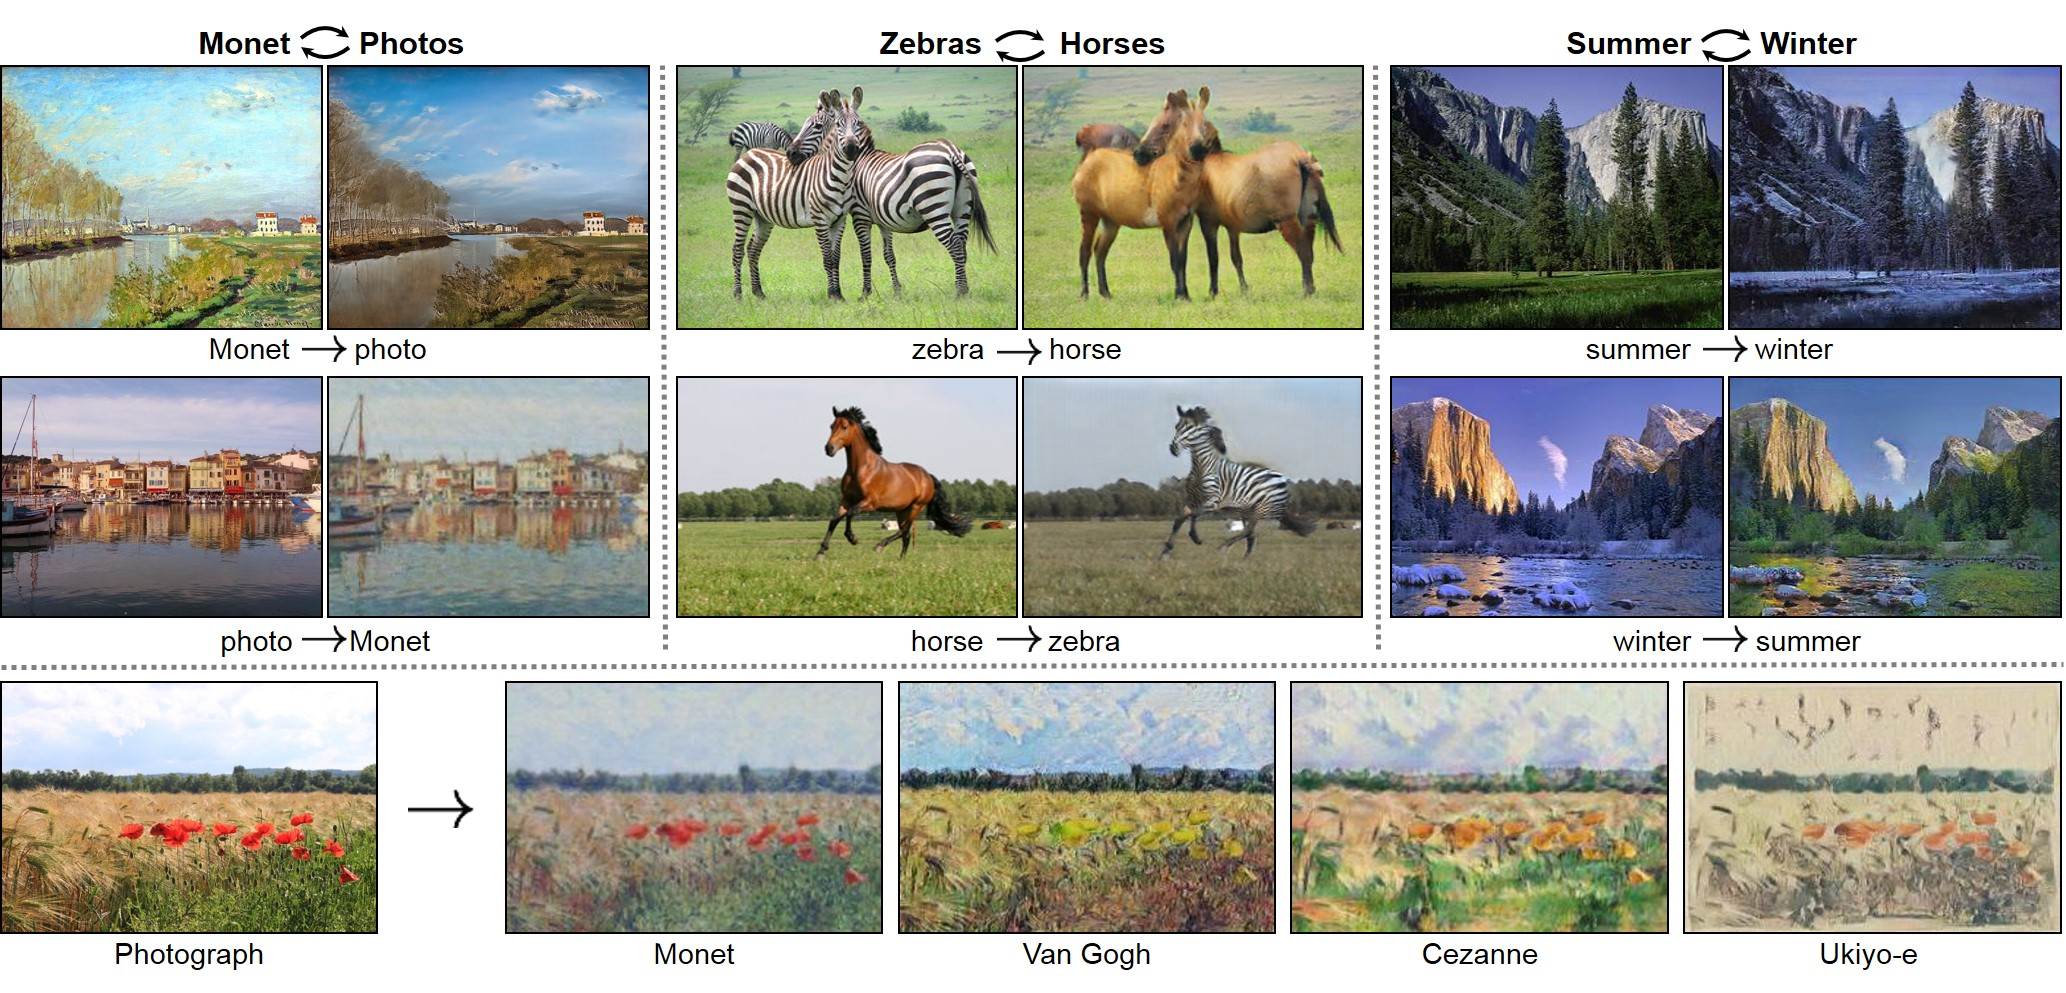
\includegraphics[width=\linewidth]{images/cyclegan.jpg}
			\caption{Pildi muundamine}
			\label{fig:cyclegan}
	\end{figure}


	CycleGAN on GAN, mis lahendab pildi pildiks teisendamise probleemi, kus soovitakse õppida seos sisendpildi ning väljundpildi vahele, näiteks teisendades mustvalgepilt värviliseks pildiks või teisendades õhufoto kaardiks. Varasemad meetodid on ainult töödanud olukordades, kus on olemas pildipaarid. Nende kogumine on aga kallis ning keeruline, mille tõttu on valmis andmekogumid pildipaaridest väikesed. CycleGANiga on võimalik õppida seos sisend- ning väljundpildi vahel isegi olukordades, kus puudub andmekogum pildipaaridest. 

	Teisendamise edukaks toimiseks peab siiski olema kahe pildi domeeni vahel mingisugune seos või struktuur. Kui proovida teisendada kassi pilte klaveri piltideks, siis on küsitav, mis on seos, mida GAN proovib õppida. Sellisel juhul ei suuda CycleGAN tihti ära õppida seost kahe pildi hulga vahel.

	Kui on antud sisend pildikogum $ X $ ja väljund pildikogum $ Y $, siis eesmärk on leida selling seos $ G: X \rightarrow Y $, et genereetitud pilt $ \hat{y} = G(x), x \in X $ oleks eristamatu pildist $ y \in Y $. Selleks kasutatakse vastast(diskrimineerijat) $ D $, mis on treenitud eristama $ y $ $ \hat{y} $-st. 

	Sellise lähenemisega kerkivad esile teatud probleemid --- antud seos ei kindlusta, et $ x $ ja $ y $ oleksid paari seatud tähendusrikkal viisil, kuna on olemas lõpmatult palju seoseid $ G $, mis loovad sama jaotuse üle $ \hat{y} $. Peale selle on raske optimeerida ainuüksi klassikalise GANi eesmärk funktsiooni, kuna see võib viia mudeli kokku varisemiseni, kus kõik sisendipildi langevad kokku ühe väljundpildiga ning optimatsioon ei suuda parandada tulemust.

	Probleeme aitab lahendada põhimõtte, et teisendus peab olema tsükliliselt järjepidev. Teisisõnu, kui tõlkida lause eesti keelest inglise keelde ning seejärel tagasi, siis peaks jõudma tagasi algse lauseni. Selle rakendamiseks on vaja kahte teisendust --- olgu esimene teisendus $ G: X \rightarrow Y $ ja teine teisendus $F: Y \rightarrow X $, siis peaksid $ G $ ja $ F $ olema üksteise pöördfunktsioonid. Et seos oleks tsükliliselt järjepidev, lisandub klassikalise GANi eesmärgile, mis treenib $ G $ ja $ F $, eesmärk, mis motiveerib tsüklilist järjepidevust $ F(G(x)) \approx x $ ja $ G(F(y)) \approx y $.

	\begin{equation}
		\loss_{cyc}(G,F) = \EX_{\boldsymbol{x}\sim p_{andmed}(\boldsymbol{x})}[\norm{F(G(\boldsymbol{x})) - \boldsymbol{x}}_1] + \EX_{\boldsymbol{y}\sim p_{andmed}(\boldsymbol{y})}[\norm{G(F(\boldsymbol{y})) - \boldsymbol{y}}_1]
	\end{equation}

	Seega täiseesmärk on:

	\begin{equation}
		\loss(G, F, D_x, D_y) = \loss_{GAN}(G, D_y, X, Y) + \loss_{GAN}(F, D_x, Y, X) + \lambda \loss_{cyc}(G, F)
	\end{equation}

	kus $ D_y $ on $ G $ diskriminaator, mis proovib eristada $ G(\boldsymbol{x}) $ ja $ \boldsymbol{y} $, $ D_x $ on  $ F $ diskriminaator, mis proovib eristada $ F(\boldsymbol{y}) $ ja $ \boldsymbol{x} $, ning $ \lambda $ on hüperparameeter, mis määrab, kui oluline on $ \loss_{cyc} $ täiseesmärgi juures.

	\subsection{Mudel}
	Selle töö poolt välja pakkutud mudel koosneb kahest komponendist --- AttnGANist, mis muudab sisendteksti pildiks, ning CycleGANist, mis muudab AttnGANi poolt loodud pildi kunstipäraseks. Lisaks sisendtekstile, määratakse ära, missuguse stiili CycleGAN pildi teisendab.

	AttnGAN ja CycleGAN mudelite jaoks kasutati vundamendina nende tööde autorite poolt kirjutatud koodi, et hoida kokku aega ning vältida vigade tekket koodis, ning millel seejärel tehti vajalikke täiendusi ja muudatusi, et sobituda kokku töö eesmärgiga.

	Et hoida kokku aega ning arvutiressursse, kasutas autor AttnGANi jaoks varem treenitud mudeleid, kuna AttnGAN ümbertreenimine ei oleks kudagi parandanud väljapakkudud mudeli sooritust.

	CycleGANi puhul tuli iga stiili jaoks ning parameetri muutmise korral treenida uus mudel. Kokku treeniti \_\_\_\_\_ mudelit, kus igat ühte treeniti ligikaudu 40 tundid RTX 2080 graafikakaardiga. Kahjuks jõudis autor treenida CycleGAN tegema \_\_\_\_\_ erinevat stiiliteisendust, aga tulevikus on plaan lisada veel teisigi stiiliteisendusi.

	Töö kood ning treenitud mudelid, mida on võimalik ka oma arvutis jooksutada, on kättesaadavad gitlabis.

	\section{Eksperimendid}
	Selles peatükkis hinnatakse välja pakutud mudeli edukust realistliku kunsti geneerimisel ning selle sisu kooskõla sisendtekstiga.

	\subsection{Andmekogud}
	AttnGAN treenimiseks kasutati CUB\parencite{cub} ja COCO\parencite{srgan} andmekogusid. CUB on andmekogum lindudest, kus on $\approx$ 10 000 pilti, kus iga pildi kohta on 10 erinevat kirjeldust. COCO on laiahaardelisem andmekogum, kus on pilte loomadest, sõidukitest, toidust ning mitmetest muudest objektidest. Andmekogus on $\approx$ 80 000 pilti, kus iga pildi kohta on 5 erinevat kirjeldust.

	CycleGANi treenimiseks kasutati Wikiart'i andmekogumit\parencite{wikiart}. Tegu on andmekoguga, kus on $\approx$ 80 000 erinevat kunstiteost, millele on juurde lisatud stiil, žanr, autor jne. Selle asemel, et andmeid uuesti kokku korjata, kasutas autor Tan jt poolt varasemalt kokku korjatud Wikiart andmekogumit\parencite{artgan}. Treenimiseks kasutati kategooriaid abstraktne ekspressionism, \_\_\_\_\_\_\_\_ ja impressionism.

	\subsection{CUB}
	Tulemustest on näha, et genereeritud pildid näevad lindude moodi välja ning samas säilitavad ka kunstistiilile iseloomulikud jooned.

	\subsection{COCO}
	Mudelil oli raskusi sellest andmekogumist pilte genereerida. Kuna kogus on pilte mitmetest erilaadi objektitest, on CycleGANil raskusi stiili ülekandmisega.

	Võib tähelda veel, et AttnGAN poolt genereeritud pildid ei ole nii realistlikud kui CUB andmekogumi puhul. Selle tõttu on erinev pildijaotuses, mida kasutati CycleGANi treenimiseks, pildijaotusest, millele CycleGAN kannab stiili üle. Pildijaotus lõhe vähendamiseks kasutati COCO testimis andmekogu 5000 erinevat kirjeldust, et genereerida 5000 uut pilti. Kasut

	Katsetasin veel lambda väärtuse muutmisega võrrandis ...

	Notes: \\
	Lisa pildijaotuse erinevuse kohta pilt

	\unsection{Kokkuvõte}
	Uurimistöö eesmärk oli luu mudel, mis oleks ise võimeline genereerima kunsti. 

	Probleemid

	Püstitatud hüpotees leidis kinnitust.

	Treenimiseks kulus palju aega.

	Autor õppis töö käigus palju uut

	\unsection{Summary}

	% The bibliography
	\nocite{*} % List all entries, even when not cited
	\printbibliography[title={Kasutatud allikad}]

\end{document}
